\documentclass{article}           %% ceci est un commentaire (apres le caractere %)
\usepackage[utf8]{inputenc}     %% adapte le style article aux conventions francophones
\usepackage[francais]{babel}
\usepackage{graphicx}

\title{Conception Détaillée\\
Tétris}     %% \title est une macro, entre { } figure son premier argument
\author{Duchesne Lucas}        %% idem

\makeindex		    %% macro qui permet de générer l'index
\bibliographystyle{prsty}	  %% le style utilisé pour créer la bibliographie
\begin{document}                  %% signale le début du document

\maketitle                        %% produire à cet endroit le titre de l'article à partir des informations fournies ci-dessus (title, author)
\newpage
\tableofcontents                  %% produire à cet endroit la table des matièree					
\newpage
\section{Introduction}            %% un titre de niveau 1 qui sera inclus dans la table des matières

Ce manuel décrira comment le code a été pensé pour pouvoir le réutiliser ultérieurement. Ainsi, nous allions étudier en premier lieu la conception générale du tétris grâce à des diagrammes UML afin d' avoir une idée générale du logiciel que nous allons présenter.
Par la suite, nous étudierions plus en détail le code pour décrire chaque détail de la programmation du logiciel. Pour cela, nous allons décrire classe par classe le code java et l’expliquer. 
L'ordre de description des classes sera approximativement celle de l'exécution du programme.

Tetris est un jeu vidéo de puzzle conçu en 1984 par Alekseï Pajitnov. Bâti sur des règles simples et exigeant intelligence et adresse, il est l'un des jeux vidéo les plus populaire au monde.

Des pièces de couleur et de formes différentes descendent du haut de l'écran. Le joueur ne peut pas ralentir ou empêcher cette chute mais peut l'accélérer ou décider à quel angle de rotation (0, 90, 180, 270) et à quel emplacement latéral l'objet peut atterrir. Lorsqu'une ligne horizontale est complétée sans vide, elle disparaît et les blocs supérieurs tombent. Si le joueur ne parvient pas à faire disparaître les lignes assez vite et que l'écran se remplit jusqu'en haut, il est submergé et la partie est finie.

\section{UML et conception}

\subsection{Présentation du projet}
Avant de commencer la description de la conception post programmation du logiciel, nous allons expliciter les spécifications du logiciel voulues dans le cahier des charges.

Nous voulons créer un tétris avec les fonctionnalités normalement établies dans un tétris comme décrit en introduction. Mais nous voulons implémenter une autre version tétris pour des fins d'utilisations pour voir comment les personnes réagissent pendant une partie de tétris. Pour cela, nous voulons pouvoir déplacer les pièces du tétris avec une précision de l'ordre du pixel et une rotation au degré prêt. De plus, nous aimerions pouvoir enregistrer les mouvements d'une partie pour pouvoir la rejouer plus tard, l'analyser, et, pour affecter les décisions des utilisateurs nous voudrions pouvoir tout modifier, tels qu'avoir plus qu'une seule couleur jusqu’à pouvoir commencer le tétris avec des briques déjà en place en bas de l'espace de jeu.


\subsection{Conception}
Les choix du langage, java, et de la librairie graphique, swing, étant suggérés dans le cahier des charges nous les  avons utilisés . Pour programmer le tétris, nous voulions une conception permettant l’extension future du logiciel. Pour cela, nous sommes partis sur une conception du logiciel sur la base vue, modèle et contrôleur, qui seront standard pour pouvoir les ré-implémenter facilement chacune séparément et sans avoir à retoucher les autres pour que logiciel fonctionne.

Cette conception sera implémentée en trois classe abstract, la classe model sera compensée des fonctions pour gérer la gestion du jeu, la classe view pour afficher les données du jeu, la classe controleur permettant de gérer les événements de l'utilisateur pour le jeu. De plus, nous avons pensé à une classe en plus pour gérer les trois autres tels le montre le graphique suivant :


\begin{figure}[h]
   \caption{Les classes de base de notre tétris}
   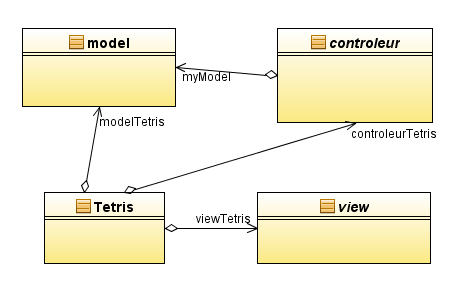
\includegraphics{diagram1.png}
\end{figure}

Le jeu tétris est basé sur la gestion de carré sur un tableau avec des carrés qui forment le décor et d'autres qui forment les pièces du tétris qui tombent. Nous avons donc pensé à gérer ces carrés à l'aide d'une classe carré permettant de définir les détails de chaque carré de l’écran tels que leurs positions et leurs couleurs. Ainsi pour gérer la pièce descendante, nous avons pensé à une classe tétrominos permettant de gérer cette dernière avec les fonctions s’effectuent dessus et un tableau de carre pour définir la pièce. Et pour définir le tableau de jeu, nous avons défini un tableau de carre dans la classe model.
Le jeu a besoin de créer les tétrominos de différents moyens pour cela nous avons pensé à une classe, \emph{terominosFactory}  implémentent différentes méthodes, soit pour la création aléatoire des tétrominos soit la création suivant une liste donné en paramètre de notre logiciel.

\begin{figure}[h]
   \caption{Les classes tétrominos, carre et model }
   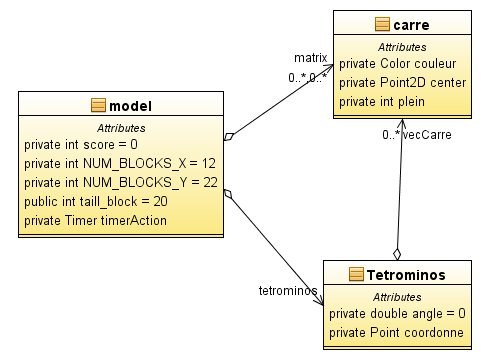
\includegraphics{diagram2.png}
\end{figure}

\newpage

L'affichage choisit pour ce logiciel et l'utiliation de la bibliothéque \emph{Swing} de java pour cela nous avons besoin de réuttiliser les classe jFrame et  jPanel permettant l'affichage de notre tétris grâce à des fenêtres de base. De plus, ces classes en java permettant de capeter les actions de l'utilisateur sur notre logiciel que ce soit mouvement de la souris, touche du clavier...
Il faudra donc que notre controleur, pour la souris, permet de récupérer ces valeurs et pour la classe view permette d'utilisé le \emph{jPanel}. Nous avons donc décidé de faire la classe principale \emph{tétris} héritant de la classe \emph{jframe} permettant ainsi d'etre notre classe principale et de relié le controleur, model et vue. Les actions, ainsi capté, ferons appel aux fonctons abstract de la classe \emph{controleur}. 
Pour le problème de l'affichage, nous devons réimplémenter la classe \emph{view} et a classe \emph{jPanel}, ici en java, nous avons choisi de faire une classe \emph{panel} héritant de la classe \emph{view}   et contenant en variable une classe \emph{persoPanel} héritant de la classe \emph{jPanel}.

\begin{figure}[]
   \caption{Les classes view et controleur en Swing }
   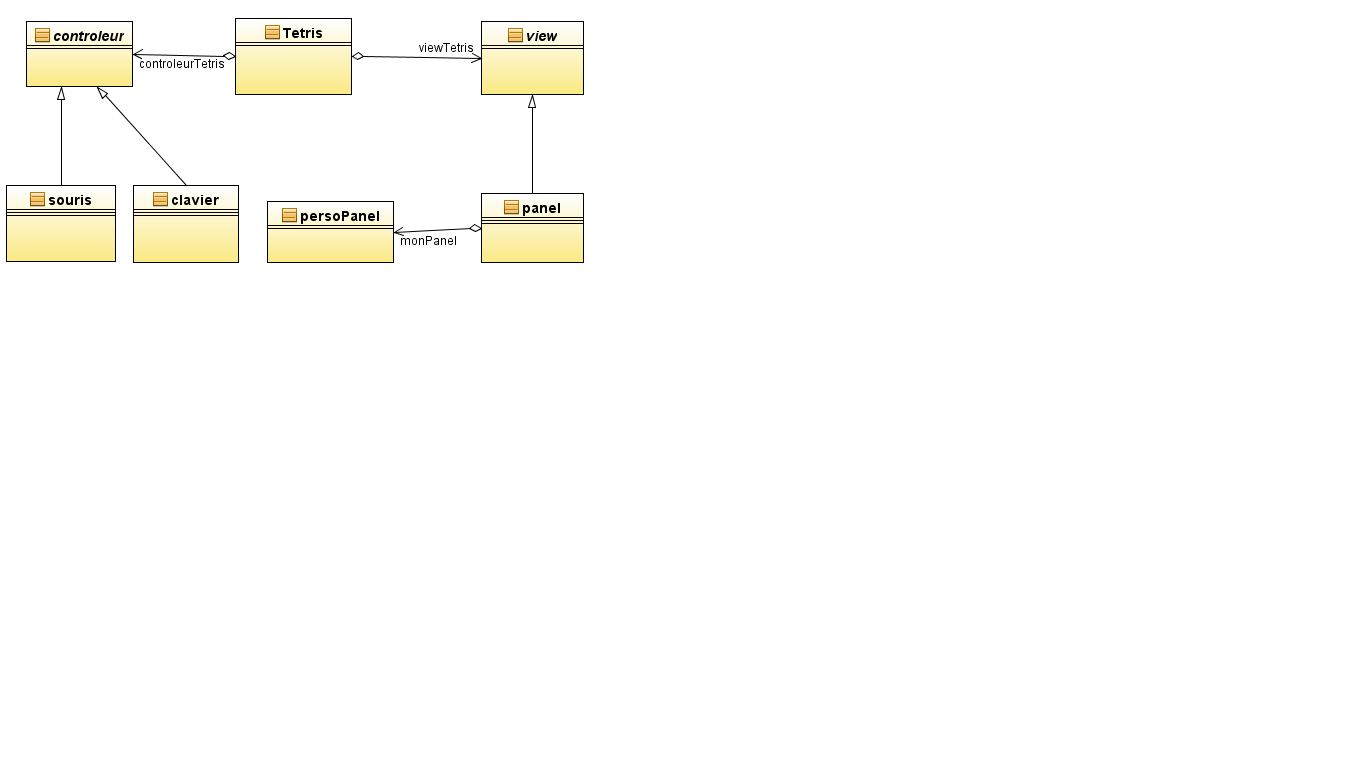
\includegraphics{diagram3.png}
\end{figure}

\newpage
Pour notre logiciel, nous avons besoin de sauvegarder les données de jeu pour pouvoir rejouer la partie dans le besoin, pour cela, nous avons besoin d'une classe qui nous permetteras de sauegarder les actions \emph{savFile} et une classe permettant de les lires \emph{lecterSeq}. Cette dernière sera une classe déduit de la classe controleur car nous la considérons comme un controleur gérant le jeu comme la souris ou le clavier.

\begin{figure}[]
   \caption{Les classes savFile et lecterSeq}
   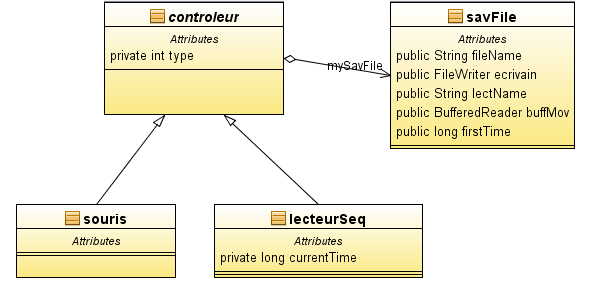
\includegraphics[width=15cm]{diagram4.png}
\end{figure}

\newpage
\section{La classe main et option}
Nous allons ici présenter la classe main, la première classe au début du programme, elle permet de gérer la fenêtre \emph{option} et de lancer une partie de tétris.

\begin{figure}[h]
   \caption{Les classes main et option détaillé }
   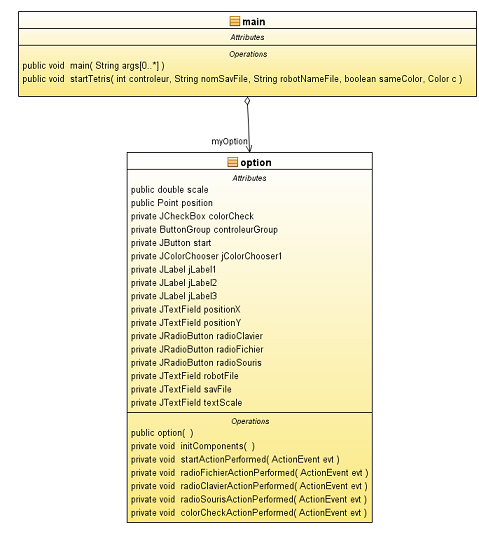
\includegraphics{diagramMain.png}
\end{figure}

La fonction principale de la classe main et \emph{startTatris} permettant d'intensifier la classe Tétris pour la partie avec les options donnée en paramètre. Elle lance le timer \emph{timerAction} principales de la partie, gérant la chute de la pièce ou la lecture du fichier de sauvegarde.

Nous avons créer la classe \emph{option} héritant de la classe \emph{Jframe} pour pouvoir avoir une interface. Dans cette dernière, nous avons rajouté différents boutons, ratio bouton, des zones de texte (pour la sauvegarde et la lecture de fichier) et le choix de couleur.
La fonction principale s'active lors du clic sur le bouton \emph{start} de la fenêtre \emph{option}. Elle appelle la fonction \emph{startTetris} de la classe \emph{main}.

\section{La classe Tétris}
Pour programmer le tétris j'ai suivi le model : view, controleur et model et c'est trois classes sont abstract de façon à pouvoir les implémenter de différents moyens si vient le besoin de changer l'interface, le controleur et model pour une évolution du logiciel futur.
Cette classe hérite de la classe Jframe pour permettre d'avoir un affichage en swing que l'on utilisera dans la classe view. Elle a comme attribut un model \emph{modelTetris}, une view \emph{viewTetris}, un model \emph{controleurTetris} et ainsi que le timer d'affichage \emph{timerAffichage} et le timer de la souris \emph{timerSouris} qui sert à effectuer une action pendant le temps ou l'utilisateur presse un bouton de la souris.

Le \emph{timerAffichage} va appeler la fonction \emph{afficher} de la classe \emph{view} tous les 50 ms pour afficher le jeu à l'écran.

\subsection{La classe Model}
La classe \emph{model} permet de gérer la gestion du jeu par rapport aux éléments reçu par la classe \emph{controleur} et de stocker les données du jeu tétris.
Nous allons parlez d'abord des attributs de cette classe et ainsi de comment sont stockées nos données de jeux. Pour cela j'ai stocké le tableau de jeux dans un tableau de classe \emph{carre} à deux dimensions de taille fixe permettant de décrire le plateau de jeu appelé \emph{matrix}. On stock une instance de la classe \emph{Tétrominos} pour savoir quelle pièce on utilise et ou la positionnée.
Le timer stocké \emph{timerAction} permet de gérer la descente de la pièce lors du choix du jeu à la souris ou autre contrôleur ou d'effectuer la prochaine action lors de la lecture du fichier enregistré.
La classe \emph{model} a les principales fonctions du jeu :

\emph{DeplacerTetrominosX} : permet de déplacer le \emph{tétrominos} courant, ou plutôt le coordonnée haut gauche du \emph{tétrominos} en considérant que le \emph{tétrominos} est dans un carré de 4x4 case. Pour cela nous appelons la fonction \emph{mettreAJourX} de la classe \emph{tétrominos}.

\emph{DeplacerTetrominosY} : Fair pareil que la fonction précédant mais sur les coordonnées X et tests si on peut encore déplacer la pièce dans le cas contraire appel la fonction \emph{placer} de \emph{tétrominos}.

\emph{rotationTetrominos} : permets de faire la rotation de la pièce courante en testant si la rotation peut se faire dans ce cas-là, on appelle la fonction \emph{rotation} de la classe \emph{tétrominos}.

\emph{testFinDeligne} : permet de tester s'il existe des lignes complètes et de les supprimer du tableau de jeu. Pour cela, elle va tester toutes les lignes en partant du bas jusqu'à ce qu'elle trouve une ligne complètement ligne.

\subsubsection{La classe Tétrominos}
La classe \emph{Tetrominos} permet de gérer chaque pièce et de stocker leur position sur le plateau. Pour cela j'ai eu besoin de stocker plusieurs variables pour cette classe.
Pour savoir sa position j'ai crée un point fictif, pour chaque tétrominos, en haut à gauche d'un carré de 4x4 \emph{carre} et on stocke cette positon dans la variable \emph{coordonne} de type \emph{Point}. Pour connaitre la composition du tétrominos j'ai stocké dans un liste de types \emph{ArrayList<carre>} nommé \emph {vecCarre} et la classe \emph {carre} permet de positionner chaque carré par rapport au centre du tétrominos. On garde aussi en mémoire l'angle de rotation dans la variable\emph{angle}.

La classe a comme fonction principale, \emph{testDeplacement} qui permet de tester si le tétrominos peut se déplacer à cette position sur le plateau. Pour cela, elle va tester pour chaque \emph{carre} du plateau si elle touche une \emph{carre} du tétrominos actuelle avec la fonction \emph{intersects} de la classe \emph{rectangle} implémenté par la classe \emph{carre}.

La fonction \emph{placer} est une fonction principale qui permet de placer la pièce sur le plateau de jeu. Pour cela, en premier lieu elle remet la pièce à l'endroit si la pièce n'est pas dans une rotation normale du jeu tétris, après rotation de la pièce on vérifie si on ne peut pas déplacer la pièce encore dans ce cas la, on rend la main à l'utilisateur. Dans l'autre cas, on met les \emph{carre} de la pièce dans le tableau à l'endroit où sont les \emph{carre} de \emph{vecCarre}.

Les autres fonctions \emph{mettreAJourX}, \emph{mettreAJourY} et \emph{rotation} permet de déplacer et d'effectuer la rotation du tétrominos pour cela on parcours chaque carre du vecteur et on déplace les coordonnées de chaque \emph{cassse} ou de faire la rotation avec la fonction \emph{rotationCenter} de \emph{carre}.

\paragraph{La classe tetrominosFactory}
Cette classe permet de gérer la création des tétrominos de différents moyens possibles. J'ai créé la fonction de telle façon qu'elle gére la gestion de différents types de création pour savoir quel type de création on est on stocke dans la variable \emph{modeCreation}. Les différents types de création ont chaque une fonction pour une création aléatoire \emph{randTetrominos}, on doit préalablement spécifier un fichier de sauvegarde de la séquence pour pouvoir rejouer la partie avec la fonction \emph{setNameFileSav} et pour la création par rapport à une séquence enregistré \emph{seqTetrominos}.
Pour cette dernière on doit spécifié le nom du fichier à lire avec la fonction \emph{setNameFileSeq}.

La fonction \emph{setTetrominos} permet de crée un tétrominos du type passé en paramètre et le renvoie.

\subsubsection{La classe carre}
Cette classe permet de gérer chaque case du jeu. Pour cela elle extends la classe \emph{rectangle} pour avoir facilement la gestion graphique et des déplacements des cubes sur le jeu.
J'ai stocké en plus comme variable la couleur du cube \emph{couleur}, une variable pour savoir si le carré est plein \emph{plein} et une variable de type \emph{Point2D} pour stocker le centre du carre. Les fonctions principales de cette classe sont :

\emph{rotationCenter}: permet de faire la rotation du \emph{carre} grâce à la fonction \emph{AffineTransform} qui va effectue la transformation du de la variable \emph{center}.

\emph{changerCoordonne}: permet de faire la translation du \emph{carre} grâce à la fonction \emph{translate} de la classe \emph{rectangle}.

\emph{changeCarre}: permet de déplacer un \emph{carre} lorsque on veut descendre une ligne.

\subsection{La classe Controleur}
La classe \emph{controleur} est une classe abstract qui permet d'implémenter les différents contrôleurs du tétris plus facilement. J'ai développé cette classe de façon quel garde en variable la classe \emph{savFile} qui contient le nom du fichier de sauvegarde des commandes et qui permet d'effectué des actions dessus. Elle garde aussi en variable le type de contrôleur utilisé lors de la section dans la variable \emph{type}.

La principale fonction est \emph{gestionTouche} qui est abstract et qui permet de l'utiliser lors du développement des différents types de contrôleur.

\subsubsection{La classe souris}
Cette classe implémente la classe \emph{controleur}, elle permet de gérer les déplacements de la souris. Comme on a développé le programme sous \emph{swing} pour capter les mouvements de la souris on l'a mis dans la \emph{tétris} qui est notre \emph{Jframe} principale et qui en revient par la création des trois fonctions suivant dans la classe \emph{tétris} : \emph{formMousePressed}, \emph{formMouseMoved} et \emph{formMouseReleased}.

La fonction \emph{formMouseMoved} permet de récupéré les coordonnées de la souris lors du déplacement et de l'envoyé à la fonction \emph{gestionTouche} de la classe \emph{souris}. Cette dernière va appeler la fonction \emph{deplacerTetrominosX} du \emph{model} avec en paramètres la position selon X de la souris.

Les fonctions emph{formMousePressed} et \emph{formMouseReleased} permettent de gérer le clique de la souris. La première s'activera lorsque qu'on cliquera sur un des boutons (bouton droit tourné à droite et inversement pour le gauche), elle déclenchera un timer qui effectuera dans chaque un des cas l'appel de la fonction \emph{rotation} du \emph{model} et sauvegardera le mouvement dans le fichier de la classe \emph{savFile} tous les 100 ms.

\subsubsection{La classe lecteurSeq}
Cette classe implémente la classe \emph{controleur}, elle permet de gérer la lecture d'un fichier de jeu et d' effectuer la partie enregistrer. Pour cela, elle va charger le fichier voulu dans la classe \emph{savFile} lors de la création de l'instance de la classe.

J'ai implémenté la fonction \emph{gestionTouche} de la classe \emph{controleur} pour quel gère la lecture du fichier, pour cela elle appelle la fonction \emph{getNextMove} de la classe \emph{savFile} qui permet de récupérer la prochain mouvement écrit dans le fichier sauvegarde et d'appeler la fonction correspondante dans la classe \emph{model} pour quel rejoue la partie sauvegardée.

Cette fonction implémentée, sera appelée dans le \emph{timerAction} tous les 10 ms, comme on a sauvegardé le temps pour chaque action on pourra modifier cet appel pour que cela puisse effectuer le jeu sauvegardé en temps normal en effectuant toutes les actions passées entre chaque 10 ms.


\subsection{La classe View}
La classe \emph{view} est une classe qui permet d'implémenter les différentes vues de notre \emph{tétris} dans le cas où l'on voudra avoir différents affichages. Cette classe a comme fonction abstract \emph{afficher} qui est appeler pour afficher le tétris. Dans notre cas, on l'implémente pour qu'elle puisse utiliser la bibliothèque \emph{Swing} du java.

\subsubsection{La classe panel}
Pour implémenter l'affichage en \emph{Swing} nous avons besoin d'implémenter la classe \emph{JPanel} et aussi \emph{view} pour notre programme. Pour cela, cette fonction fera la liaison entre l'implémentation des deux. Elle a comme variable \emph{monPanel} qui est de type \emph{persoPanel} qui n'est d'autre n'autre implémentation du \emph{Jpanel}.

\emph{afficher} est implémenté dans cette classe pour appeler le \emph{repaint} de la classe \emph{persoPanel}

\subsubsection{La classe persoPanel}
Cette classe permet d'implémenter la classe \emph{jPanel} pour avoir un affichage en \emph{swing}. Cette classe a comme variable \emph{matrix} et \emph{tetrominos} pour savoir ce qui faut afficher et la variable \emph{sameColor} qui permet de savoir si l'affichage doit se faire avec une seule couleur.

\section{Conclusion}               %% un autre titre

En conclusion, le programme implémente les fonctions essentielles du cahier des charges :

\begin{enumerate}
  \item Reproduction du comportement du jeu standard 
  		\begin{enumerate}
		  \item Même pièce, les 7 pièces différentes, \textbf{Oui}.	
		  \item Même actions = tourner/déplacer/tomber, \textbf{Oui}.
		  \item Possibilité de mettre en pause, \textbf{Non}.
		\end{enumerate}

  \item Déplacement avec une précision arbitraire des pièces, \textbf{Oui}.
  \item Rotation avec précision arbitraire, \textbf{Oui}.
  \item Contrôle du jeu à la souris, \textbf{Oui}, la classe \emph{souris}.
  \item Contrôle du jeu au clavier, \textbf{Non}, classe existante mais pas implémenté.
  \item Gestion des conflits entre commandes de l'utilisateur et contraintes du jeu, \textbf{Oui}, la fonction \emph{tetrominos.testDeplacement()}.
  \item Recaler les Tetrominoes sur la grille des blocs une fois qu'ils sont stabilisés/tombés, \textbf{Oui}, la fonction \emph{tetrominos.placer()}.
  \item Détermination de la séquence des Tetrominoes, \textbf{Oui}, la classe \emph{tetrominosFactory}.
  \item Sauvegarde du comportement de l'utilisateur, \textbf{Oui}, la classe \emph{savFile}.
  \item Contrôle du jeu directement depuis un fichier de données, \textbf{Oui}, la classe \emph{lecteurSeq}.
  \item Limitation possible de la vitesse maximale de déplacement des Tetrominos, \textbf{Oui}.

 \end{enumerate}

Le code corespond aux exigences techniques voulues : 

\begin{enumerate}
	\item Implémentation en Java, \textbf{Oui}.	
	\item Interface graphique Swing, \textbf{Oui}.
	\item Finalisation sous forme de package exécutable avec code source intégré, \textbf{Oui}.
	\item Indépendance à des bibliothèques/packages sont standards , \textbf{Oui}.
	\item Modèle de conception permettant de produire plusieurs vues/contrôles, \textbf{Oui}.
	\item Rendre le code le plus modulaire et extensible possible, \textbf{Casi}.
\end{enumerate}
 											 

\end{document} 